\section{溶解度}\label{sec:4-3}

\subsection{饱和溶液和不饱和溶液}

在一定条件下,溶质是不是可以无限制地溶解在一定量的溶剂里呢?

\begin{shiyan}\label{shiyan:4-4}
    在各盛有 10 毫升水的两个试管里,分别缓缓地加入食盐和硝酸钾的固体。
    边加入,边振荡,到试管里的固体有剩余,再不能溶解为止(保留试管里的溶液,
    供下面的实验用)。这个实验说明了什么问题?
\end{shiyan}

实验说明,在一定温度下(实验是在室温下做的),食盐和硝酸钾虽然都能溶解于水,
但在一定量的水里,食盐和硝酸钾溶解的量是一定的,不能无限制地溶解。

我们把在一定温度下,在一定量的溶剂里,
不能再溶解某种溶质的溶液叫做这种溶质的\zhongdian{饱和溶液};
还能继续溶解某种溶质的溶液,叫做这种溶质的\zhongdian{不饱和溶液}。
例如在上面的实验里,在室温下当食盐或硝酸钾还能继续溶解的时候,试管里的溶液是不饱和溶液;
当食盐或硝酸钾不能继续溶解而有固体剩余的时候,试管里的溶液就是饱和溶液了。

为了粗略地表示溶液里溶质含量的多少,通常把溶液区分为浓溶液和稀溶液。
浓溶液和稀溶液只指溶液中溶质含量的多少,不管溶液是饱和的或是不饱和的。
有些难溶物质(如熟石灰)在水里即使溶解很少一点儿,溶液虽然很稀,可是已经达到饱和了。
相反地,有些易溶物质(如蔗糖)即使溶解了许多,溶液虽然很浓,却还没有达到饱和。
因此,应当明确认识浓溶液不一定是饱和溶液,稀溶液不一定是不饱和溶液。
当然对于同一种溶质的溶液,在一定温度时,饱和溶液比不饱和溶液浓一些是对的。

在讲饱和溶液和不饱和溶液时, 为什么一定要指出 “一定温度” 和 “一定量的溶剂” 呢?

\begin{shiyan}\label{shiyan:4-5}
    给实验 \ref{shiyan:4-4} 里盛有剩余食盐固体的试管缓缓加入少量的水,边加入,边振荡,
    观察溶液里剩余的食盐固体有什么变化?

    给实验 \ref{shiyan:4-4} 里有硝酸钾固体的试管缓缓加热,边加热,边振荡,
    观察溶液里剩余的硝酸钾固体有什么变化
    (保留试管里的溶液,供下面的实验用)。
\end{shiyan}

从上面的实验可以看到,
给盛有剩余食盐的试管里加水时,原来不能再溶解的食盐又能继续溶解了;
给盛有剩余硝酸钾的试管加热时,原来不能再溶解的硝酸钾也能继续溶解了。
可见在增加溶剂的量或升高温度的情况下,这些饱和溶液可以变成不饱和溶液。
因此,饱和溶液和不饱和溶液在改变条件时,可以互相转变。
只有指明在 “一定温度” 下和在 “一定量的溶剂” 里,
“饱和” 和 “不饱和” 才具有确定的意义。


\subsection{固体的溶解度}

在相同的条件下,有些物质容易溶解在水里,有些物质很难溶解,这是我们熟悉的事实。
可见,不同的物质在同一溶剂里,溶解的能力各不相同。
通常把一种物质溶解在另一种物质里的能力叫做溶解性。
溶解性的大小跟溶质和溶剂的性质有关。例如,
食盐容易溶解在水里,但是很难溶解在汽油里;
油脂很难溶解在水里,但是很容易溶解在汽油里。
我们通常用溶解度来表示物质的溶解性。
\zhongdian{在一定温度下,某物质在 100 克溶剂里达到饱和状态时所溶解的克数,
叫做这种物质在这种溶剂里的溶解度。}
如果不指明溶剂,通常所说的溶解度就是物质在水里的溶解度。
例如,在 20 ℃ 时,氯酸钾的溶解度是 7.4 克,食盐的溶解度是 36 克。

各种物质在水里的溶解度是不同的。
通常把在室温(20 ℃)时溶解度在 10 克以上的,叫易溶物质;
溶解度大于 1 克的,叫可溶物质;
溶解度小于 1 克的,叫微溶物质;
溶解度小于 0.01 克的,叫难溶物质。
绝对不溶于水的物质是没有的。习惯上把难溶物质叫做 “不溶” 物质。
例如,在 20 ℃,碳酸钙的溶解度是 0.0013 克,所以把碳酸钙叫做 “不溶” 物质。
溶解是绝对的,不溶只是相对的。所谓易溶、可溶、微溶、难溶或不溶都是相对而言的。

当温度发生变化的时候,物质的溶解度有没有变化呢?

\begin{shiyan}
    实验 \ref{shiyan:4-5} 里盛有硝酸钾溶液的试管放置稍久,冷却后又有硝酸钾晶体析出,
    然后再加热,硝酸钾固体又溶解了。在加热了的溶液里继续加入硝酸钾,
    到不能再溶解为止。等溶液冷却后,观察有什么现象发生。
\end{shiyan}

从上面的实验可以看到,在加热的时候,原来在室温下已经达到饱和的硝酸钾溶液又可以继续溶解硝酸钾,
也就是说,随着温度的升高,硝酸钾的溶解度增大了;但是,这种在较高温度下达到饱和的溶液冷却以后,
部分已溶解的硝酸钾又成为固体硝酸钾,也就是说,随着温度的降低,硝酸钾的溶解度减小了。

我们可以用实验的方法,测出硝酸钾在各种温度时在水里的溶解度,见表 \ref{tab:4-1}。

\begin{table}[htbp]
    \centering
    \caption{硝酸钾在各种不同温度的溶解度}\label{tab:4-1}
    \begin{tblr}{
        hlines, vlines,
        columns={mode=math, c},
        column{1}={mode=text}
    }
        温度(℃)  & 0    & 10   &  20  & 30   & 40   & 50   & 60    & 70  & 80  & 90  & 100 \\
        溶解度(克)& 13.3 & 20.9 & 31.6 & 45.8 & 63.9 & 85.5 & 110.0 & 138 & 169 & 202 & 246
    \end{tblr}
\end{table}

我们用纵坐标表示溶解度,横坐标表示温度,根据硝酸钾在不同温度时的溶解度,
可以画出硝酸钾的溶解度随温度变化的曲线,这种曲线叫做\zhongdian{溶解度曲线}。
用同样方法,也可以画出其它固体物质的溶解度曲线(图 \ref{fig:4-2}) 。

\begin{figure}[htbp]
    \centering
    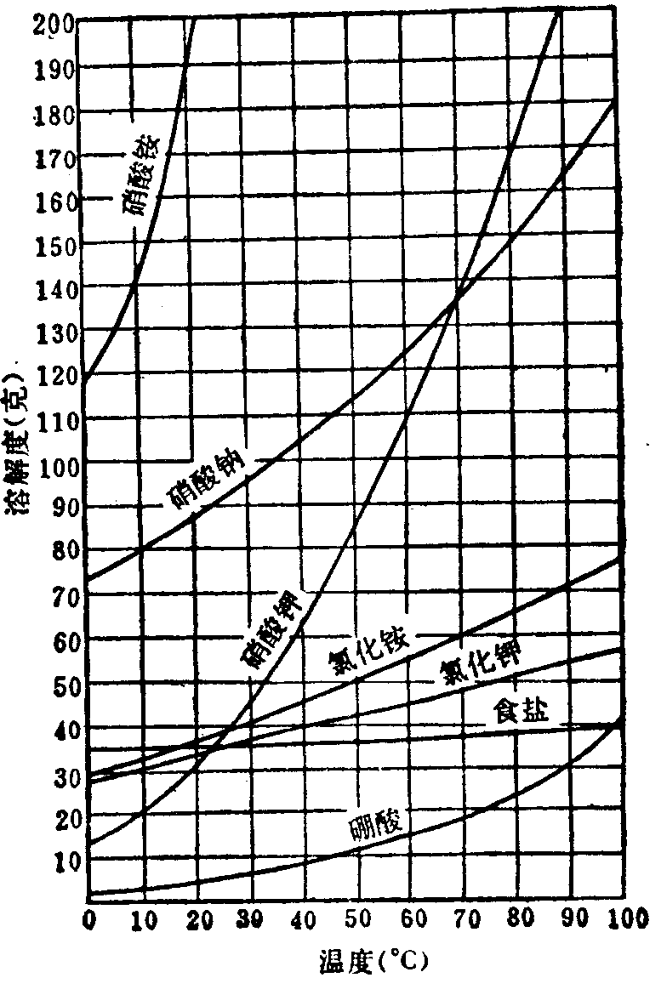
\includegraphics[width=8cm]{../pic/czhx1-ch4-2}
    \caption{固体的溶解度曲线}\label{fig:4-2}
\end{figure}

利用溶解度曲线,也可以求出物质在不同温度的溶解度。
例如,氯化铵在 10 ℃ 的溶解度是 33.3 克;在 80 ℃ 的溶解度是 65.6 克。
食盐在 10 ℃ 的溶解度是 35.8 克;在 80 ℃ 是 38.4 克。

我们在比较了各种物质在水里的溶解度后知道,大部分固体物质的溶解度随着温度的升高而增大。
例如,硝酸钾、氯化铵。只有少数物质的溶解度受温度的影响很小。例如食盐。
也有极少数物质的溶解度随着温度的升高而减小。例如熟石灰(图 \ref{fig:4-3}) 。

\begin{figure}[htbp]
    \centering
    \begin{minipage}[b]{9cm}
        \centering
        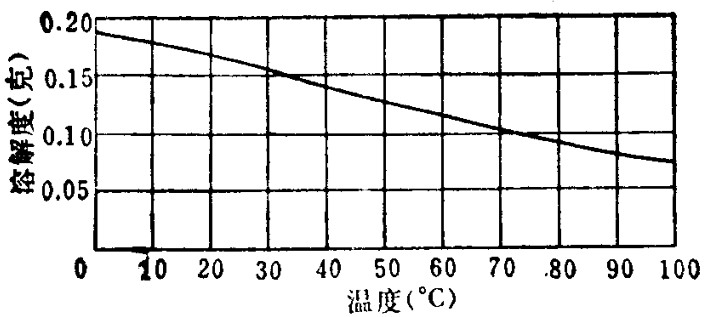
\includegraphics[width=8cm]{../pic/czhx1-ch4-3}
    \caption{熟石灰的溶解度曲线}\label{fig:4-3}
    \end{minipage}
    \qquad
    \begin{minipage}[b]{5.5cm}
        \centering
        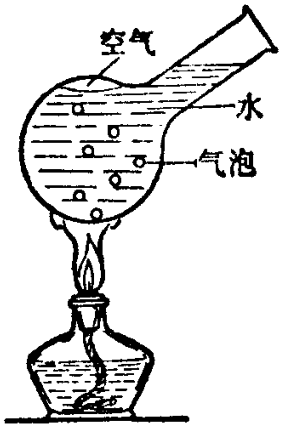
\includegraphics[width=4cm]{../pic/czhx1-ch4-4}
        \caption{气体溶解度跟温度的关系}\label{fig:4-4}
    \end{minipage}
\end{figure}


\subsection{气体的溶解度}

当我们打开汽水瓶瓶盖时,看到溶解在水里的二氧化碳(\ce{CO2}) 气体,形成气泡由瓶口逸出,这是什么原因呢?

这是因为气体在水里的溶解度,不仅决定于气体的性质,还决定于气体的压强的大小。
当温度不变时,随着压强的增大,气体的溶解度也增大。
在制汽水时,就是把二氧化碳气体的压强增大,使二氧化碳气体在水里的溶解度增大。
当打开汽水瓶盖的时候,压强减小了,溶解度也减小了,因此,有大量的二氧化碳气体由水里逸出。


温度对气体的溶解度也有很大的影响。气体的溶解度一般随着温度的升高而减小。
例如,给冷水加热的时候,随着温度的升高,原来溶解在水里的空气在水沸腾以前,就形成气泡放出,如图 \ref{fig:4-4} 所示。

由于称量气体的质量比较困难,所以气体溶解度通常指的是该
气体\footnote{非标准状况时的气体体积数要换算成标准状况时的体积数。}(其
压强为 1 标准大气压)在一定温度时溶解在 1 体积的水里的体积数。例如,
在  0 ℃ 时,氮气的溶解度为 0.024,氧气为 0.049,
在 20 ℃ 时,氮气的溶解度为 0.015,氧气为 0.031 等等。



\subsection{关于溶解度的计算}

1. 根据在某一定温度时某种物质的饱和溶液里的溶质和溶剂的质量,可以计算这种物质的溶解度。


\liti 把 50 克 20 ℃ 的硝酸钾饱和溶液蒸干,得到 12 克硝酸钾,求硝酸钾在 20 ℃ 的溶解度。

\jie 50 克硝酸钾溶液里含有 38 克水($50 \; \ke - 12\; \ke$)。

设 100 克水里溶解 $x$ 克硝酸钾。
\begin{align*}
    38:12 &= 100:x \\
    x = \dfrac{12 \times 100}{38} &= 31.6 \; (\ke)
\end{align*}

答:硝酸钾在 20 ℃ 的溶解度等于 31.6 克。


2. 已知某物质在某一温度时的溶解度,可以计算出在一定量的饱和溶液里某物质的质量。

\liti 根据溶解度曲线,计算在 20 ℃ 时 1000 克氯化铵饱和溶液里含氯化铵多少克。

\jie 根据溶解度曲线,在 20 ℃ 时氯化铵的溶解度是 37.2 克。
即 137.2 克氯化铵饱和溶液里含有 37.2 克氯化铵。

设 1000 克氯化铵饱和溶液里含有 $x$ 克氯化铵。
\begin{align*}
    137.2:37.2 &= 1000:x \\
    x = \dfrac{37.2 \times 1000}{137.2} &= 271.1 \; (\ke)
\end{align*}

答: 在 20 ℃ 时, 1000 克氯化铵饱和溶液里含有 271.1 克氯化铵。


3. 已知某物质在某一温度时的溶解度,可以计算出一定量的溶质配制成饱和溶液时,所需水的质量。

\liti 已知 20 ℃ 时食盐的溶解度是 36 克。在 20 ℃ 时要把 40 克食盐配制成饱和的食盐水,需要水多少克?

\jie 从题意可知在 20 ℃ 时 36 克食盐跟 100 克水恰好能配制成食盐的饱和溶液。

设 20 ℃ 时, 40 克食盐配制成食盐的饱和溶液需要水 $x$ 克
\begin{align*}
    100:36 &= x:40 \\
    x = \dfrac{100 \times 40}{36} &= 111.1 \; (\ke)
\end{align*}

答:在 20 ℃ 时, 40 克食盐配制成饱和溶液需要用水 111.1 克。


\begin{xiti}

\xiaoti{现有一瓶接近饱和的硝酸钾溶液,试举出使它成为饱和溶液的两种方法。}


\xiaoti{下列说法是否正确?为什么?}
\begin{xiaoxiaotis}

    \xxt{20 ℃ 时, 把 10 克食盐溶解在 100 克水里, 所以 20 ℃ 时食盐的溶解度是 10 克。}

    \xxt{20 ℃ 时, 100 克食盐溶液里含有 10 克食盐,所以 20 ℃ 时食盐的溶解度是 10 克。}

\end{xiaoxiaotis}


\xiaoti{设有 A 、B、 C 三种物质,在 20 ℃ 时分别溶解在水里制成饱和溶液。已知
    A 物质 1   克溶解在 10   克水里;
    B 物质 150 克溶解在 1000 克水里;
    C 物质 25  克溶解在 350  克水里,哪一种物质的溶解度大?
}

\xiaoti{已知 30 ℃ 时,氯酸钾的溶解度是 10 克。
    把 30 ℃ 时配制成的 44 克氯酸钾饱和溶液蒸干后,可得到氯酸钾多少克?
}

\xiaoti{在 70 ℃ 时, 45 克氯化铵饱和溶液中含有多少克氯化铵?\\
    (提示: 氯化铵的溶解度可由图 \ref{fig:4-2} 查得。)
}

\xiaoti{要配制 50 ℃ 的氯化钾饱和溶液(50 ℃ 时氯化钾的溶解度是 42.6 克)。}
\begin{xiaoxiaotis}

    \xxt{25 克氯化钾应溶解在多少克的水里?}

    \xxt{在25 克水里能溶解多少克氯化钾?}

\end{xiaoxiaotis}


\xiaoti{在 18 ℃ 时,溶解 27 克碳酸钾至少需要水多少克?
    如果溶解在 50 克水中,应再加多少克碳酸钾才能成为饱和溶液?
    ( 在18 ℃ 时,碳酸钾的溶解度是108 克。)
}

\end{xiti}

